%%%%%%%%%%%%%%%%%%%%%%%%%%%%%%%%%%%%%%%%%
% Beamer Presentation
% LaTeX Template
% Version 1.0 (10/11/12)
%
% This template has been downloaded from:
% http://www.LaTeXTemplates.com
%
% License:
% CC BY-NC-SA 3.0 (http://creativecommons.org/licenses/by-nc-sa/3.0/)
%
%%%%%%%%%%%%%%%%%%%%%%%%%%%%%%%%%%%%%%%%%

%----------------------------------------------------------------------------------------
%    PACKAGES AND THEMES
%----------------------------------------------------------------------------------------

\documentclass{beamer}

\mode<presentation> {
	
	% The Beamer class comes with a number of default slide themes
	% which change the colors and layouts of slides. Below this is a list
	% of all the themes, uncomment each in turn to see what they look like.
	
	%\usetheme{default}
	%\usetheme{AnnArbor}
	%\usetheme{Antibes}
	%\usetheme{Bergen}
	%\usetheme{Berkeley}
	%\usetheme{Berlin}
	%\usetheme{Boadilla}
	%\usetheme{CambridgeUS}
	%\usetheme{Copenhagen}
	%\usetheme{Darmstadt}
	%\usetheme{Dresden}
	%\usetheme{Frankfurt}
	%\usetheme{Goettingen}
	%\usetheme{Hannover}
	%\usetheme{Ilmenau}
	%\usetheme{JuanLesPins}
	%\usetheme{Luebeck}
	\usetheme{Madrid}
	% \usepackage{listings}
	%\usetheme{Malmoe}
	%\usetheme{Marburg}
	%\usetheme{Montpellier}
	%\usetheme{PaloAlto}
	%\usetheme{Pittsburgh}
	%\usetheme{Rochester}
	%\usetheme{Singapore}
	%\usetheme{Szeged}
%	\usetheme{Warsaw}
	
	% As well as themes, the Beamer class has a number of color themes
	% for any slide theme. Uncomment each of these in turn to see how it
	% changes the colors of your current slide theme.
	
%	\usecolortheme{albatross}
%	\usecolortheme{beaver}
%	\usecolortheme{beetle}
%	\usecolortheme{crane}
%	\usecolortheme{dolphin}
%	\usecolortheme{dove}
%	\usecolortheme{fly}
%	\usecolortheme{lily}
%	\usecolortheme{orchid}
%	\usecolortheme{rose}
%	\usecolortheme{seagull}
%	\usecolortheme{seahorse}
%	\usecolortheme{whale}
%	\usecolortheme{wolverine}
	
%	\setbeamertemplate{footline} % To remove the footer line in all slides uncomment this line
	%\setbeamertemplate{footline}[page number] % To replace the footer line in all slides with a simple slide count uncomment this line
	
%	\setbeamertemplate{navigation symbols}{} % To remove the navigation symbols from the bottom of all slides uncomment this line
	\usefonttheme{serif}
}
\usepackage{graphicx,wrapfig,lipsum}
\usepackage{graphicx} % Allows including images
\usepackage{booktabs} % Allows the use of \toprule, \midrule and \bottomrule in tables
\usepackage{wrapfig}

\usepackage{subcaption}
\usepackage{tikz}
\usetikzlibrary{decorations.pathmorphing,matrix,decorations.pathreplacing,arrows,decorations.markings}
\usetikzlibrary{fit,calc,shapes,arrows,positioning,shadings,backgrounds,patterns,tikzmark,matrix,spy}
\usetikzlibrary{decorations.markings}

\tikzset{myrow/.style args = {(#1,#2)}{%
		row #1/.style={nodes={fill=#2}}}}

\tikzset{mycolumn/.style args = {(#1,#2)}{%
		column #1/.style={nodes={fill=#2}}}}

\tikzset{mycell/.style args = {(#1,#2,#3)}{%
		row #1 column #2/.style={nodes={fill=#3}}}}

\makeatletter
\usetikzlibrary{chains,patterns,shadows}
\tikzset{% customization of pattern
	% based on <m.wibrow@gm...> - 2013-03-24 07:20: 
	hatch distance/.store in=\hatchdistance,
	hatch distance=5pt,
	hatch thickness/.store in=\hatchthickness,
	hatch thickness=5pt
}
\pgfdeclarepatternformonly[\hatchdistance,\hatchthickness]{north east hatch}% name
{\pgfqpoint{0pt}{0pt}}% below left
{\pgfqpoint{\hatchdistance}{\hatchdistance}}% above right
{\pgfpoint{\hatchdistance-1pt}{\hatchdistance-1pt}}%
{
	\pgfsetcolor{\tikz@pattern@color}
	\pgfsetlinewidth{\hatchthickness}
	\pgfpathmoveto{\pgfqpoint{0pt}{0pt}}
	\pgfpathlineto{\pgfqpoint{\hatchdistance}{\hatchdistance}}
	\pgfusepath{stroke}
}

\newcommand{\KECCAK}{\mbox{\textsc{Keccak}}}
\newcommand{\Keccak}{\mbox{\textsc{Keccak}}}
\newcommand{\SHA}{\textsc{Sha}}
\newcommand{\Rnd}{\textsc{Round}}
\newcommand{\etal}{\textit{et al. }}
%----------------------------------------------------------------------------------------
%    TITLE PAGE
%----------------------------------------------------------------------------------------

\title[Cryptanalysis of Round Reduced \KECCAK{}]{Cryptanalysis of Round Reduced \KECCAK{}} % The short title appears at the bottom of every slide, the full title is only on the title page

\author{Nikhil Mittal} % Your name
\institute[17111056] % Your institution as it will appear on the bottom of every slide, may be shorthand to save space
{
	Under supervision of\\
	\medskip
	{\large Prof. Manindra Agrawal and Dr. Shashank Singh}\\
	\medskip
	IIT Kanpur \\ % Your institution for the title page
	\medskip
	\textit{nickedes@cse.iitk.ac.in} % Your email address
}
\date{June 13, 2019} % Date, can be changed to a custom date
% \documentclass[border=10pt]{standalone}

\begin{document}
%	\setbeamertemplate{caption}{\raggedright\insertcaption\par}
	
	\begin{frame}
	\titlepage % Print the title page as the first slide
\end{frame}

%\begin{frame}
%\frametitle{Table of Contents}
%\tableofcontents
%\end{frame}

\section{Introduction}

\begin{frame}
	\frametitle{Hash Function}
	\begin{itemize}
		\item A hash function is a deterministic function of the form $H:\{0,1\}^* \rightarrow \{0,1\}^n $.
		\medskip
		\item It takes as input an arbitrary string (of $0$'s and $1$'s) and outputs a fixed size (say $n$) string.
		\medskip
		\pause
		\item It is used in many cryptographic applications e.g., Authentication, Digital Signatures and Integrity etc..
	\end{itemize}
\end{frame}

\begin{frame}
	\frametitle{Cryptographic Hash Functions}
	\begin{itemize}
		\item Cryptographic applications require hash functions to satisfy the following conditions:\\
		\begin{itemize}\setlength\itemindent{10pt}
			\pause
			\item {\bf Efficiency}: Given a message $m$, it is easy to compute its hash i.e. $H(m)$.\\
			\medskip
%			\pause
			\item {\bf Preimage Resistance}: Given $H(m)$, it is computationally hard to find the message $m$.\\
			\medskip
%			\pause
			\item {\bf Second-preimage Resistance}: Given a message $m$, it is computationally hard to find another message $m^\prime$ such that $H(m)=H(m^\prime)$.\\
			\medskip
%			\pause
			\item {\bf Collision Resistance}: It is computationally hard to find two messages $m$ and $m^\prime$ such that $H(m)=H(m^\prime)$.\\
		\end{itemize}
		\pause
		\item Hash functions having the above properties are referred to as cryptographic/secure hash functions.
	\end{itemize}
\end{frame}

\begin{frame}
	\frametitle{Need For \SHA-$3$}
	\begin{itemize}
		\item MD$5$, \SHA-$1$, \SHA-$2$ are very popular hash functions and are widely used.
%		\pause
		\item In year 2005, first practical collision attacks were found on:
		\begin{itemize}
			\item MD$5$, \SHA-$0$ and \SHA-$1$ by Xiaoyun Wang \etal.
		\end{itemize}
		
%		\item In the year $2005$, the first practical collision attack on MD$5$ was published by Xiaoyun Wang \etal
%		\item in the same year, a practical collision attack on \SHA-$0$ and \SHA-$1$ was published by Xiaoyun Wang \etal
%		\pause
		\item National Institute of Standards and Technology (NIST) was worried about the security of hash functions.
		
		\item Though by that time \SHA-$2$ family of hash functions was standardized.
%		\pause
		\item \SHA-$2$ was also based on Merkle-Damgard construction like \SHA-$0$, \SHA-$1$.
		\item There was a possibility that it could also be attacked in a similar fashion.
	\end{itemize}
\end{frame}

\begin{frame}
	\frametitle{\SHA-$3$ Competition}
	\begin{itemize}
		\item In the year $2006$, NIST decided to hold a competition for the next secure hash function.
		\medskip
%		\pause
		\item In $2008$, NIST announced a competition for the Secure Hash Algorithm-$3$ (\SHA-$3$).
				\medskip
%		\pause
		\item  In the year $2012$, NIST announced \KECCAK{} as the winner of the competition among the five finalists viz. BLAKE, Gr\o stl, JH, \KECCAK{} and Skein.
%				\medskip
%		\pause
		\item Since $2015$, \KECCAK{} has been standardized as \SHA-$3$ by NIST.
		
	\end{itemize}
\end{frame}

\begin{frame}
	\frametitle{\KECCAK{}}
	\begin{itemize}
		\item \KECCAK{} hash function is based on sponge construction.
				\medskip
		\item \SHA-$3$ family of hash functions is based on \Keccak{}.
				\medskip
		\item The \SHA-$3$ family provides four hash functions:
			\begin{itemize}
				\item \SHA3-$224$, \SHA3-$256$, \SHA3-$384$ and \SHA3-$512$.
			\end{itemize}
				\medskip
		\pause
		\item \Keccak{}'s excellent resistance towards crypt-analytic attacks is one of the main reasons for its selection by NIST.
				\medskip
		\item The algorithm is a good mixture of linear as well as non-linear operations.
	\end{itemize}
\end{frame}

\begin{frame}
	\frametitle{Sponge Construction}
	\begin{itemize}
		\item A sponge construction consists of:
			\begin{itemize}
				\item Permutation function $f$,
				\item Parameter ``rate'' $r$, and
				\item Padding rule pad.
%				\pause
				\item This construction produces a sponge function that takes as input a bit string $M$ and generates a string of length $l$.
			\end{itemize}
	\end{itemize}
	\begin{figure}
	\resizebox{250pt}{!}{
		\includegraphics[scale=0.5]{sponge.png}
	}
	\caption{\textcolor{blue}{The sponge construction}\label{sponge}}
\end{figure}
\end{frame}

\begin{frame}
	\begin{itemize}
		\frametitle{\KECCAK{}-$p$ Permutation}
		\item The function $f$ in the sponge construction is denoted by \KECCAK-$f\left[b\right]$.
				\medskip
		\item $b$ is the length of input string.
				\medskip
		\item Internally, \KECCAK-$f\left[b\right]$ consists of a round function $p$ which is applied $n_r$ number of times.
				\medskip
		\item \KECCAK-$f\left[b\right]$ function is specialization of \KECCAK-$p\left[b, n_r\right]$.
	\end{itemize}
\end{frame}
		
\begin{frame}
	\frametitle{\KECCAK{} State}
	\begin{itemize}
		\item The state input to \KECCAK-$f\left[b\right]$ consists of $b$ bits.
		\item The state is divided into slices.
		\item Each slice is of fixed size i.e., $25$ bits.
		\item A state $S$, which is a $b$-bit string, in \Keccak{} is usually denoted by a $3$-dimensional grid of size $(5 \times 5 \times w)$.
		\begin{figure}
			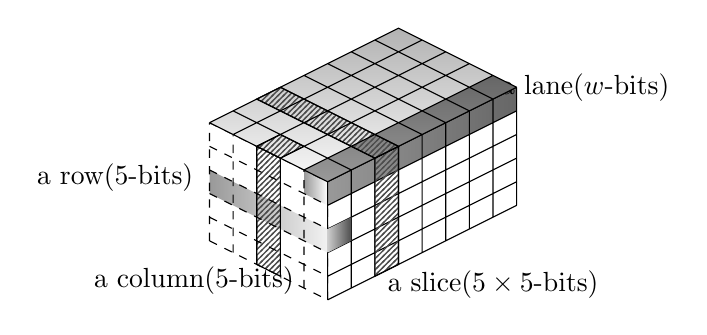
\begin{tikzpicture}[on grid,scale=0.3]
				\shade[yslant=-0.5,right color=gray!10, left color=black!40] (0,2) rectangle +(5,1) node[xshift=-1.2cm, yshift=0.2cm] at (0,2){ a row($5$-bits)};
				%lane 1x1
				\shade[yslant=-0.5,left color=black!40,  color=black!10] (4,4) rectangle +(1,1);
				%column
				\draw[yslant=-0.5,pattern=north east hatch,  pattern color=black!70, hatch distance=3pt, hatch thickness=0.5pt] (2,0) rectangle +(1,5)
				node[xshift=-0.8cm, yshift=-0.2cm] at (2,0){ a column($5$-bits)};
				
				\draw[yslant=-0.5, dashed] (0,0) grid (5,5);
				\shade[yslant=0.5,right color=black!60,left color=black!40](5,-1) rectangle +(8,1);
				\draw[yslant=0.5] (5,-5) grid (13,0);
				\node at (15.9,6.5){a lane($w$-bits)};
				%slice front
				\draw[yslant=0.5,pattern=north east hatch,  pattern color=black!70, hatch distance=3pt, hatch thickness=0.5pt](7,-5) rectangle +(1,5)
				node[xshift=1.5cm, yshift=-0.1cm] at (7,-5){ a slice($5\times 5$-bits)};
				%row front
				\shade[yslant=0.5,left color=black!20,right color=black!70] (5,-3) rectangle +(1,1);
				%top shade
				\shade[yslant=0.5,xslant=-1,bottom color=gray!5,top color=gray!60] (5,0) rectangle +(8,5);
				\shade[yslant=0.5,xslant=-1, bottom color=black!40,top color=black!60](5,0) 
				rectangle +(8,1); 
				%slice top 
				\draw[yslant=0.5,xslant=-1,pattern=north east hatch,  pattern color=black, hatch distance=3pt, hatch thickness=0.5pt] (7,0) rectangle +(1,5);
				%column top
				\draw[yslant=0.5,xslant=-1,pattern=north east hatch,  pattern color=black, hatch distance=3pt, hatch thickness=0.5pt] (5,2) rectangle +(1,1);
				
				\draw[yslant=0.5,xslant=-1] (5,0) grid (13,5);
				\end{tikzpicture}
			\caption{\textcolor{blue}{The \KECCAK{} State}}
		\end{figure}
	\end{itemize}
\end{frame}

\begin{frame}
	\frametitle{Round Function of \KECCAK{}-$p$}
	\begin{itemize}
		\item The round function $p$ in \Keccak{} comprises of $5$ step mappings.
%		\medskip
%		\item The \Keccak{} state undergoes some transformations specified by the step mapping.
		\medskip
		\item These step mappings are called $\theta,\;\rho,\;\pi,\;\chi\;and\;\iota$.
				\medskip
		\item These transformations are applied in sequence.
				\medskip
%		\item Now, we will describe these $5$ step mappings in detail.
	\end{itemize}
\end{frame}

\begin{frame}
	\frametitle{$\theta$ step mapping}
	\begin{itemize}
		\item XOR each bit in the state with the parities of two neighboring columns.
		\pause
%		\item For bit position $\left(x,\; y,\; z\right)$, one column is $\left(\left(x - 1\right) \bmod 5,\; z\right) $ and the other is $\left(\left(x+1\right)\bmod 5,\; \left(z - 1\right) \bmod w\right)$.
%		\pause
		\item If we have $A$ as the input state to $\theta$, then the output state $B$ is:
		
		\vskip5pt
		\tikz\node[draw, rounded corners, fill=yellow!40]{\parbox{0.95\linewidth}{
		\begin{align}\nonumber
		B\left[x,\; y,\; z\right] &= A\left[x,\; y,\; z\right] \bigoplus P\left[(x - 1) \bmod 5 ,\, z \right] \\
		&\hspace{1.3cm}\bigoplus P\left[ (x + 1) \bmod 5 ,\, (z - 1) \bmod w \right]
		\end{align}
		}};	\vskip5pt
	
		where $P\left[x,\; z\right]$ represents the parity of the column $(x,\; z)$ i.e.,
		\[
		P\left[x,\; z\right]  = \bigoplus_{y = 0}^{4} A\left[x,\; y,\; z\right]
		\]
	\end{itemize}
\end{frame}

\begin{frame}
	\frametitle{$\rho$ step mapping}
	\begin{itemize}
		\item $\rho$ ({\bf rho}): This step rotates each lane by a constant value towards the MSB.
				\medskip
		\pause
		\item If we have $A$ as the input state to $\rho$, then the output state $B$ is given by:\vskip5pt
		\begin{center}
		\tikz\node[draw, rounded corners, fill=yellow!40]{\parbox{0.65\linewidth}{
		\begin{equation*}
			B\left[x, \,y,\, z\right] = A\left[x, \,y, \,z + \rho\left(x, y\right) \bmod w\; \right],
		\end{equation*}
		}};
		\end{center}
		\vskip5pt
		where $\rho\left(x,\; y\right)$ is the constant for a given lane $\left(x,\; y\right)$.
%				\medskip
%		\item The constant value $\rho\left(x,\; y\right)$ is specified for each lane in the construction of \Keccak{}.
%		\pause
				\medskip
		\item $\rho$ is a linear step mapping.
	\end{itemize}
\end{frame}

\begin{frame}
	\frametitle{$\pi$ step mapping}
	\begin{itemize}
		\item $\pi$ ({\bf pi}): It permutes the position of lanes.
				\medskip
		\item The new position of a lane is determined by a matrix, 
	\begin{center}
		\tikz\node[draw, rounded corners, fill=yellow!40]{\parbox{0.55\linewidth}{
		\begin{align}
		\begin{bmatrix} x'\\ y'\end{bmatrix} = 
		\begin{bmatrix} $0$ & $1$ \\ $2$ &  $3$ \end{bmatrix} \cdot \begin{bmatrix} x\\ y\end{bmatrix},
		\end{align}
	}};
	\end{center}
		where $\left(x',\; y'\right)$ is the position of lane $\left(x,\; y\right)$ after $\pi$ step.
				\medskip
		\item $\pi$ is also a linear step mapping.
	\end{itemize}
\end{frame}

\begin{frame}
	\frametitle{$\chi$ step mapping}
	\begin{itemize}
		\item $\chi$ ({\bf chi}): Each bit in the original state is XOR-ed with a non-linear function of next two bits in the same row.
		\vskip5pt
		\begin{center}
			\tikz\node[draw, rounded corners, fill=yellow!40]{\parbox{0.97\linewidth}{
		\begin{align}\nonumber
		&B[x,\; y,\; z] =  A[x,\; y,\; z] \;\oplus \\
		& \hspace{0.5cm} \left( \left(A[ (x + 1 )\bmod 5,\; y,\; z] \oplus 1\right) \cdot  A[ (x + 2) \bmod 5,\; y,\; z] ) \right).
		\end{align}
		}};
		\end{center}
		\vskip5pt
%		\pause
		\item $\chi$ is the only non-linear operation among the $5$ step mappings in \KECCAK{}.
	\end{itemize}
\end{frame}

\begin{frame}
	\frametitle{$\iota$ step mapping}
	\begin{itemize}
	    \item $\iota$ ({\bf iota}): This step mapping only modifies the $(0,\;0)$ lane depending on the round number.
	    
	    \item If we have $A$ as the input state to $\iota$, then the output state $B$ is:
		\begin{align}
			B[0,\; 0] = A[0,\; 0] \oplus RC_i,
		\end{align}
		where $RC_i$ is round constant that depends on the round number.
%		\pause
		\item The remaining $24$ lanes remain unaffected.	
%		\pause
		\item All the rounds are identical but the symmetry is destroyed by this step due to the addition of a round constant to a particular lane.
	\end{itemize}
\end{frame}

\begin{frame}
	\frametitle{Specification of \KECCAK-$p\left[ b, n_r \right]$}
	\begin{itemize}
		\item Round in \Keccak{} is given by:
		\medskip
		\begin{itemize}
			\item ${\tt Round}\left(A,\; i_r\right) = \iota\left( \chi\left( \pi \left( \rho \left( \theta \left( A \right) \right) \right) \right),\; i_r\right)$
		\end{itemize}
		\medskip
		\item It consists of $n_r$ number of iterations of ${\tt Round}\left(A,\; i_r\right)$.
		\medskip
		\item \KECCAK-$p\left[ b,\;n_r \right] \left( S \right)$
			\begin{itemize}
				\item Convert $S$ into a state array $A$
				\medskip
				\item For $i_r$ from $0$ to $n_r - 1$, let $A = {\tt Round}\left(A,\; i_r\right)$
				\medskip
				\item Convert $A$ into string $S'$ of length $b$
				\medskip
				\item Return $S'$
			\end{itemize}
	\end{itemize}
\end{frame}

\begin{frame}
	\frametitle{\SHA-$3$ Hash Function}
	\begin{itemize}
		\item The \SHA-$3$ hash function is \Keccak-$p\left[b,\; 12 + 2\cdot l\right]$.
		\item $w = b/25$ and $l = \log_{2}\left(w\right)$
		\pause
		\item When the value of $b = 1600$, we have $l = 6$.
		\item Thus, the $f$ function in \SHA-$3$ is \Keccak-$p\left[1600,\; 24\right]$.
		\pause
		\item Instances of \Keccak{} are denoted by $\Keccak\left[r,\;c\right]$.
		\item Where $r=b-c$ and the capacity $c$ is chosen to be twice the size of hash output $d$.
		\pause
		\item We set $c = 2\cdot d$, to avoid generic attacks with expected cost below $2^d$.
		\item The hash function with output length $d$ is denoted by: 
		\begin{eqnarray}
		\mbox{\Keccak-$d$}  &=& \Keccak\left[r:=b-2\cdot d,\;c:=2\cdot d\right]
		\end{eqnarray}
	\end{itemize}
\end{frame}

\begin{frame}
	\frametitle{pad10*1}
	\begin{itemize}
		\item The padding rule followed by \KECCAK{} is \textbf{pad10*1}.
				\medskip
		\item According to the rule, the input string is appended with a $1$ bit followed by some number of $0$ bits and followed by $1$ bit.
				\medskip
		\item The asterisk in the padding rule indicates that $0$ bit is either not present or is repeated as required so that the length of output string after padding is a multiple of the block length (i.e. $r$).
	\end{itemize}
\end{frame}

\begin{frame}
	\frametitle{\KECCAK[r:=800-384, c:=384]}
	\begin{itemize}
		\item $\KECCAK\left[r:=800-384, c:=384\right] = \KECCAK\text{-}p\left[800,24\right]\left[r:=800-384, c:=384\right]$.\\
		\pause
		\bigskip
		\item $2$-round $\KECCAK\left[r:=800-384, c:=384\right] = \KECCAK\text{-}p\left[800,2\right]\left[r:=800-384, c:=384\right]$.
	\end{itemize}
\end{frame}

\begin{frame}
	\frametitle{Observations}
	\begin{itemize}
		\item \label{ob1}\textbf{Observation 1:} If we know all the bits of a row, then we can invert $\chi$ for that row. It is depicted below.
		%------------------------------------------------------
		\begin{figure}
			\begin{center}
				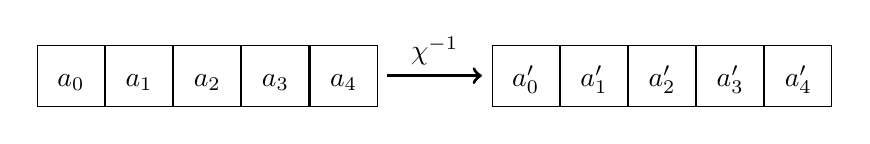
\begin{tikzpicture}[ampersand replacement=\&]
				\matrix (m1) [matrix of nodes,
				nodes={inner sep=5pt,text width=0.5cm,align=center,minimum height=.5cm, draw,text height=1em,text depth=.2em}
				]{
					$a_0$ \& $a_1$\& $a_2$ \& $a_3$ \& $a_4$\\
				};
				
				\matrix (m2) [right = 1.2cm of m1, matrix of nodes,
				nodes={inner sep=5pt,text width=0.5cm,align=center,minimum height=.5cm, draw,text height=1em,text depth=.2em}
				]{
					$a_0^\prime$ \& $a_1^\prime$\& $a_2^\prime$ \& $a_3^\prime$ \& $a_4^\prime$\\
				};
				\draw[->, very thick] (m1)-- node[above, pos=0.5] {$\chi^{-1}$} (m2);
				\end{tikzpicture}
			\end{center}
			\caption{Computation of $\chi^{-1}$ for full row \label{chi_inv}}
		\end{figure}
		%------------------------------------------------------
		% check it for correctness
		\begin{align}
		a_i^\prime = a_i \oplus \left( a_{i+1} \oplus 1\right) \cdot \left( a_{i+2} \oplus \left( a_{i+3} \oplus 1 \right) \cdot a_{i+4}\right)
		\end{align}
		
		\item \label{ob2}\textbf{Observation 2:} When only one output bit is known after $\chi$ step, then we can fix the first output bit to be the same as the input bit and the second bit as $1$. 		
		%------------------------------------------------------
		\begin{figure}[ht]
			\begin{center}
				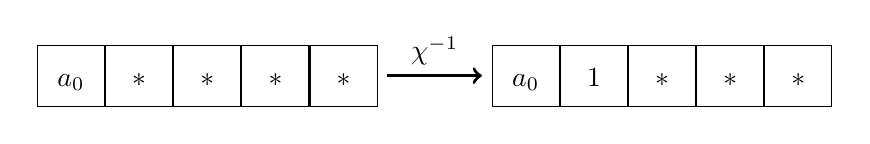
\begin{tikzpicture}[ampersand replacement=\&]
				\matrix (m1) [matrix of nodes,
				nodes={inner sep=5pt,text width=0.5cm,align=center,minimum height=.5cm, draw,text height=1em,text depth=.2em}
				]{
					$a_0$ \& $*$ \& $*$ \& $*$ \& $*$\\
				};
				
				\matrix (m2) [right = 1.2cm of m1, matrix of nodes,
				nodes={inner sep=5pt,text width=0.5cm,align=center,minimum height=.5cm, draw,text height=1em,text depth=.2em}
				]{
					$a_0$ \& $1$ \& $*$ \& $*$ \& $*$\\
				};
				\draw[->, very thick] (m1)-- node[above, pos=0.5] {$\chi^{-1}$} (m2);
				\end{tikzpicture}
			\end{center}
			\caption{Computation of $\chi^{-1}$ when only 1-bit is known in row \label{chi_inv2}}
		\end{figure}
	\end{itemize}
\end{frame}

\begin{frame}
\frametitle{Observations}
\begin{itemize}
	\item \label{ob3}\textbf{Observation 3:} 
	
	\item $a_i', \;a_i$ are the input and output bits of $\chi$ respectively.
	
	\item Guo \etal observed that when $4$ out of $5$ output bits of $\chi$ are known, then we can obtain $4$ linear relations in terms of $a_i'$.
	
	
	\begin{align}\label{eq:a0}
	a_i^\prime = a_i \oplus \left( a_{i+1} \oplus 1\right) \cdot \left( a_{i+2} \oplus \left( a_{i+3} \oplus 1 \right) \cdot a_{i+4}\right)
	\end{align}
	
	\item If the values of $a_0,\;a_1,\;a_2,\;a_3$ are known using the Equation~\ref{eq:a0}, we can eliminate the expression $a_4$ from the rest of the equations.
	\item Hence, we obtain $4$ linear equations on the input bits.
	
\end{itemize}
\end{frame}

\begin{frame}
	\frametitle{Notations}
	\begin{itemize}
		\item The \KECCAK{} state is represented by $25$ lanes.
				\medskip
		\item Each lane is represented by a variable which is a $32$-bit array.
				\medskip
		\item A variable with a number in round bracket $``\left( \cdot \right)"$ represents the shift of the bits in array towards MSB.
				\medskip
		\item A variable with a number in square bracket $``\left[ \cdot \right]"$ represents the bit value of the variable at that index. 
				\medskip
		\item If there are multiple numbers in the square bracket, then it represents the corresponding bit values.
	\end{itemize}
\end{frame}

\begin{frame}
	\frametitle{2 rounds of \KECCAK[r:=800-384, c:=384]}
	\begin{figure}
		\centering
		\includegraphics[scale=0.5]{keccak2Rstate.pdf}
		\caption{Two rounds of \KECCAK$[r:=800-384, c:=384]$}
		\label{two_rnd}
	\end{figure}
	% first one is initial state, second is intermediate state and last is final state
	\begin{itemize}
		\item We will discuss a preimage attack on above structure.
	\end{itemize}
\end{frame}

\begin{frame}
	\frametitle{Final State of 2-round \KECCAK[r:=800-384, c:=384]}
	\begin{itemize}
		\item $c = 384 \rightarrow d = 192 \rightarrow$ hash of $6$ lanes
	\end{itemize}
	\begin{figure}[ht]
		\begin{center}
			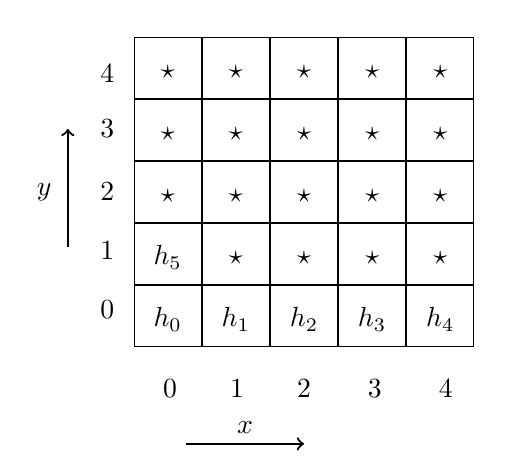
\begin{tikzpicture}[ampersand replacement=\&]
			\matrix (sm1) [matrix of nodes,
			nodes={inner sep=5pt,text width=0.5cm,align=center,minimum height=.5cm, draw,text height=1em,text depth=.2em}
			]{
				$\star$ \& $\star$\& $\star$ \& $\star$ \& $\star$\\
				$\star$ \& $\star$\& $\star$ \& $\star$ \& $\star$\\
				$\star$ \& $\star$\& $\star$ \& $\star$ \& $\star$\\
				$h_5$ \& $\star$\& $\star$ \& $\star$ \& $\star$\\
				$h_0$ \& $h_1$\& $h_2$ \& $h_3$ \& $h_4$\\
			};
			\node[] at (-1.7,-2.5) { 0 };
			\node[] at (-0.85,-2.5) { 1 };
			\node[] at (0.0,-2.5) { 2 };
			\node[] at (0.9,-2.5) { 3 };
			\node[] at (1.8,-2.5) { 4 };
			\draw[thick,->] (-1.5, -3.2) -- node [above] {$x$} (0.0, -3.2);
			\node[] at (-2.5,-1.5) { 0 };
			\node[] at (-2.5,-0.75) { 1 };
			\node[] at (-2.5,0.0) { 2 };
			\node[] at (-2.5,0.8) { 3 };
			\node[] at (-2.5,1.5) { 4 };
			\draw[thick,->] (-3, -0.7) --  (-3, 0.8);
			\node[] at (-3.3, 0) {$y$};
			\end{tikzpicture}
		\end{center}
		\caption{The Final Hash State for \KECCAK{}$\left[r:=800-384, c:=384\right]$ \label{initial_sq}}
	\end{figure}
\end{frame}

\begin{frame}
	\frametitle{Initial State of 2-round \KECCAK[r:=800-384, c:=384]}
	\begin{itemize}
		\item $r = 800 - 384 \rightarrow r = 416 \rightarrow$ Message block of $13$ lanes
	\end{itemize}
	\begin{figure}
		\begin{center}
			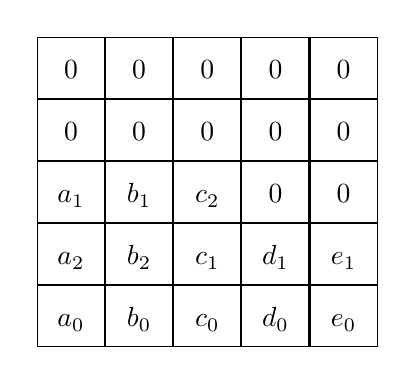
\begin{tikzpicture}[ampersand replacement=\&]
			\matrix (sm1) [matrix of nodes,
			nodes={inner sep=5pt,text width=0.5cm,align=center,minimum height=.5cm, draw,text height=1em,text depth=.2em}
			]{
				$0$ \& $0$\& $0$ \& $0$ \& $0$\\
				$0$ \& $0$\& $0$ \& $0$ \& $0$\\
				$a_1$ \& $b_1$\& $c_2$ \& $0$ \& $0$\\
				$a_2$ \& $b_2$\& $c_1$ \& $d_1$ \& $e_1$\\
				$a_0$ \& $b_0$\& $c_0$ \& $d_0$ \& $e_0$\\
			};
			\end{tikzpicture}
		\end{center}
		\caption{Setting of Initial State in the Attack}
	\end{figure}
\end{frame}

\begin{frame}
	\frametitle{Attack}
	\begin{itemize}
		\item Our aim is to find the values of $a_0,\; a_1,\; a_2$, $b_0,\; b_1,\; b_2$, $c_0,\; c_1,\; c_2$, $d_0,\; d_1$ and $e_0,\; e_1$ variables in the initial state.
		\medskip
		\pause
		\item Such that, they lead to a final state having first six lanes as $h_0,\;h_1,\;h_2,\;h_3,\;h_4$ and $h_5$.
		\medskip
		\pause
		\item We follow the basic idea of the attack given by Naya \etal in $2011$.
		\medskip
		\pause
		\item $2$ rounds of \KECCAK{}$\left[r:=800-384,\;c:=384\right]$\\
			\begin{itemize}
				\item Best-known attack, has a time complexity of $O(2^{64})$.
				\medskip
				\item It is based on the idea of linear structures given by Jian Guo \etal in $2016$.
			\end{itemize} 
	\end{itemize}
\end{frame}

\begin{frame}
	\frametitle{First round $\theta$ step mapping}
	\begin{itemize}
		\item $\theta$ step mapping diffuses message bits to full state.
		\pause
				\medskip
		\item In this step, our aim is to control the diffusion by $\theta$.
				\medskip
		\item This can be done by adding constraints on message bits.
		\pause
				\medskip
		\item We add the following conditions to make column parity zero:
		\begin{align}\nonumber
		a_2 &= a_0 \oplus a_1,\quad b_2 = b_0 \oplus b_1, \quad c_2 = c_0 \oplus c_1\\ \label{cond_state1}
		d_1 & = 0,\quad d_0 = 0\;\;\text{ and }\;\; e_1 = e_0.
		\end{align}
	\end{itemize}
\end{frame}

\begin{frame}
\frametitle{Effect of $\theta$}
\begin{figure}[!t]
	\begin{center}
		\resizebox{\textwidth}{!}{%
			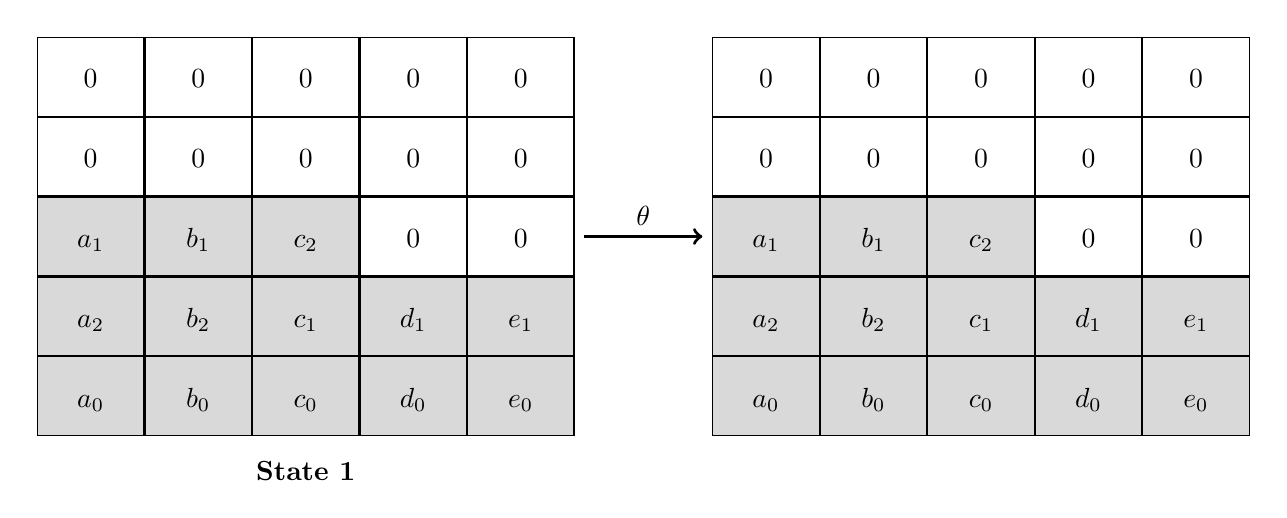
\begin{tikzpicture}[ampersand replacement=\&, scale=0.5]
			\matrix (am1) [matrix of nodes,nodes in empty cells,
			nodes={inner sep=5pt,text width=1.0cm,align=center,minimum height=1.0cm, draw,text height=1em,text depth=.2em},
			myrow/.list={(1,white),(2,white),(4,gray!30),(5,gray!30)},
			mycell/.list={(3,1,gray!30),(3,2,gray!30),(3,3,gray!30),(3,4,white),(3,5,white)}]    
			{
				$0$ \& $0$\& $0$ \& $0$ \& $0$\\
				$0$ \& $0$\& $0$ \& $0$ \& $0$\\
				$a_1$ \& $b_1$\& $c_2$ \& $0$ \& $0$\\
				$a_2$ \& $b_2$\& $c_1$ \& $d_1$ \& $e_1$\\
				$a_0$ \& $b_0$\& $c_0$ \& $d_0$ \& $e_0$\\
			};
			\matrix (am2) [right=1.5 cm of am1,matrix of nodes,nodes in empty cells,
			nodes={inner sep=5pt,text width=1.0cm,align=center,minimum height=1.0cm, draw,text height=1em,text depth=.2em},
			myrow/.list={(1,white),(2,white),(4,gray!30),(5,gray!30)},
			mycell/.list={(3,1,gray!30),(3,2,gray!30),(3,3,gray!30),(3,4,white),(3,5,white)}
			]    
			{
				$0$ \& $0$\& $0$ \& $0$ \& $0$\\
				$0$ \& $0$\& $0$ \& $0$ \& $0$\\
				$a_1$ \& $b_1$\& $c_2$ \& $0$ \& $0$\\
				$a_2$ \& $b_2$\& $c_1$ \& $d_1$ \& $e_1$\\
				$a_0$ \& $b_0$\& $c_0$ \& $d_0$ \& $e_0$\\
			};
			\node[ below=0.2cm of am1-5-3]{\bf State~1};
			\node[ below=0.2cm of am2-5-4]{};
			\draw[->, very thick] (am1)-- node[above]{$\theta$} (am2);
			
			\end{tikzpicture}
		}
		\caption{Effect of $\theta$ on initial state}
	\end{center}
\end{figure}
\end{frame}

\begin{frame}
	\frametitle{State $1$ to State $2$}
	\begin{figure}[!t]
		\begin{center}
			\resizebox{\textwidth}{!}{%
				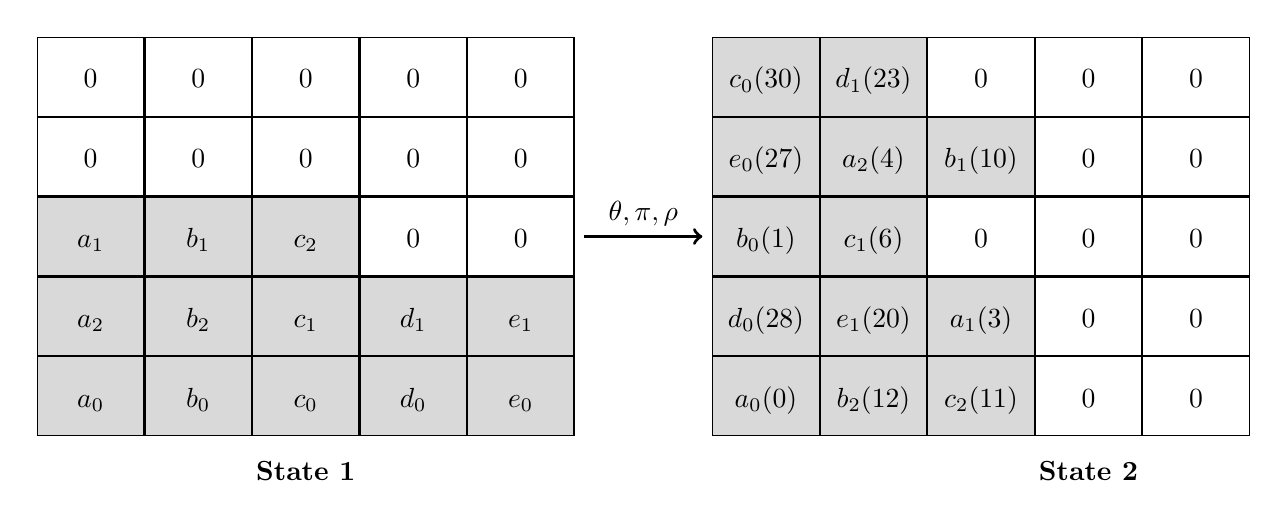
\begin{tikzpicture}[ampersand replacement=\&, scale=0.5]
				\matrix (am1) [matrix of nodes,nodes in empty cells,
				nodes={inner sep=5pt,text width=1.0cm,align=center,minimum height=1.0cm, draw,text height=1em,text depth=.2em},
				myrow/.list={(1,white),(2,white),(4,gray!30),(5,gray!30)},
				mycell/.list={(3,1,gray!30),(3,2,gray!30),(3,3,gray!30),(3,4,white),(3,5,white)}]    
				{
					$0$ \& $0$\& $0$ \& $0$ \& $0$\\
					$0$ \& $0$\& $0$ \& $0$ \& $0$\\
					$a_1$ \& $b_1$\& $c_2$ \& $0$ \& $0$\\
					$a_2$ \& $b_2$\& $c_1$ \& $d_1$ \& $e_1$\\
					$a_0$ \& $b_0$\& $c_0$ \& $d_0$ \& $e_0$\\
				};
				\matrix (am2) [right=1.5 cm of am1,matrix of nodes,nodes in empty cells,
				nodes={inner sep=5pt,text width=1.0cm,align=center,minimum height=1.0cm, draw,text height=1em,text depth=.2em},
				mycolumn/.list={(1,gray!30),(2,gray!30),(4,white),(5,white)},
				mycell/.list={(1,3,white),(3,3,white),(2,3,gray!30),(4,3,gray!30),(5,3,gray!30)}
				]    
				{
					$c_0(30)$ \& $d_1(23)$ \& $0$         \& $0$ \& $0$\\
					$e_0(27)$ \& $a_2(4)$ \& $b_1(10)$ \& $0$ \& $0$\\
					$b_0(1)$  \& $c_1(6)$  \& $0$         \& $0$ \& $0$\\
					$d_0(28)$ \& $e_1(20)$ \& $a_1(3)$  \& $0$ \& $0$\\
					$a_0(0)$  \& $b_2(12)$ \& $c_2(11)$ \& $0$ \& $0$\\
				};
				
			
				
				
				\node[ below=0.2cm of am1-5-3]{\bf State~1};
				\node[ below=0.2cm of am2-5-4]{\bf State~2};
				\draw[->, very thick] (am1)-- node[above]{$\theta, \pi,\rho$} (am2);
				
				\end{tikzpicture}
			}
			\caption{Preimage attack on $2$-round \KECCAK{}$[r:=800-384,\; c:=384]$}
		\end{center}
	\end{figure}
\end{frame}

\begin{frame}{$\chi$ and $\iota$ inverse}
\begin{figure}[!t]
	\begin{center}
		\resizebox{\textwidth}{!}{%
			\begin{tikzpicture}[ampersand replacement=\&, scale=0.5]
			
			\matrix (am3) [below=1.5 cm of am2,matrix of nodes,nodes in empty cells,
			nodes={inner sep=5pt,text width=1.0cm,align=center,minimum height=1.0cm, draw,text height=1em,text depth=.2em, fill=gray!10},
			mycell/.list={(5,1,gray!50),(5,2,gray!50),(5,3,gray!50),(5,4,gray!50),(5,5,gray!50),(4,1,gray!50),(4,2,gray!50)}
			]	
			{
				\&  	\&   	\&  	\& \\
				\&  	\&   	\& \& 		\\
				\&  	\& \&  	\& 		\\
				$h_5^\prime$ 	\& $1$ \&   	\&  	\& 		\\
				$h_0^\prime$ \& $h_1^\prime$		\& $h_2^\prime$  	\& $h_3^\prime$ 	\& $h_4^\prime$		\\
			};
			\matrix (am4) [left=1.50 cm of am3,matrix of nodes,nodes in empty cells,
			nodes={inner sep=5pt,text width=1.0cm,align=center,minimum height=1.0cm, draw,text height=1em,text depth=.2em, fill=gray!10},
			mycell/.list={(5,1,gray!50),(5,2,gray!50),(5,3,gray!50),(5,4,gray!50),(5,5,gray!50),(4,1,gray!50)}
			]	
			{
				\&  \&   \&  \& \\
				\&  \&   \&  \& \\
				\&  \&   \&  \& \\
				$h_5$ \&  \&   \&  \& \\
				$h_0$ \& $h_1$\& $h_2$ \& $h_3$ \& $h_4$\\
			};
			
			\node[ below=0.2cm of am3-5-3]{};
			\node[ below=0.2cm of am4-5-3]{\bf State~4};
			\draw[->, very thick] (am4)-- node[above, pos=0.4]{$\;\;\chi^{-1} \circ \iota^{-1}$}  (am3);
			\end{tikzpicture}
		}
		\caption{Inversion of hash through $\chi^{-1} \circ \iota^{-1}$}
	\end{center}
\end{figure}
\end{frame}


\begin{frame}
	\frametitle{State $4$ to State $3$}
	    \begin{figure}[!t]
		\begin{center}
			\resizebox{\textwidth}{!}{%
				\begin{tikzpicture}[ampersand replacement=\&, scale=0.5]
				
				\matrix (am3) [below=1.5 cm of am2,matrix of nodes,nodes in empty cells,
				nodes={inner sep=5pt,text width=1.0cm,align=center,minimum height=1.0cm, draw,text height=1em,text depth=.2em, fill=gray!10},
				mycell/.list={(5,1,gray!50),(4,2,gray!50),(3,3,gray!50),(2,4,gray!50),(1,5,gray!50),(5,4,gray!50),(4,5,gray!50)}
				]	
				{
					\&  	\&   	\&  	\& $h_4^\prime(18)$\\
					\&  	\&   	\&$h_3^\prime(11)$ \& 		\\
					\&  	\& $h_2^\prime(21)$\&  	\& 		\\
					\&$h_1^\prime(20)$ \&   	\&  	\& $1$		\\
					$h_0^\prime(0)$ \& 		\&  	\& $h_5^\prime(4)$ 	\& 		\\
				};
				\matrix (am4) [left=1.50 cm of am3,matrix of nodes,nodes in empty cells,
				nodes={inner sep=5pt,text width=1.0cm,align=center,minimum height=1.0cm, draw,text height=1em,text depth=.2em, fill=gray!10},
				mycell/.list={(5,1,gray!50),(5,2,gray!50),(5,3,gray!50),(5,4,gray!50),(5,5,gray!50),(4,1,gray!50)}
				]	
				{
					\&  \&   \&  \& \\
					\&  \&   \&  \& \\
					\&  \&   \&  \& \\
					$h_5$ \&  \&   \&  \& \\
					$h_0$ \& $h_1$\& $h_2$ \& $h_3$ \& $h_4$\\
				};
				
				\node[ below=0.2cm of am3-5-3]{\bf State~3};
				\node[ below=0.2cm of am4-5-3]{\bf State~4};
				\draw[->, very thick] (am4)-- node[above, pos=0.4]{$\iota^{-1},\chi^{-1}$} node[below, pos=0.6]{$ \pi^{-1},\rho^{-1}$} (am3);
				\end{tikzpicture}
			}
%			\caption{}
		\end{center}
	\end{figure}
\end{frame}

\begin{frame}{State 1 to 4}

\begin{figure}[!t]
	\begin{center}
		\resizebox{250pt}{!}{%
			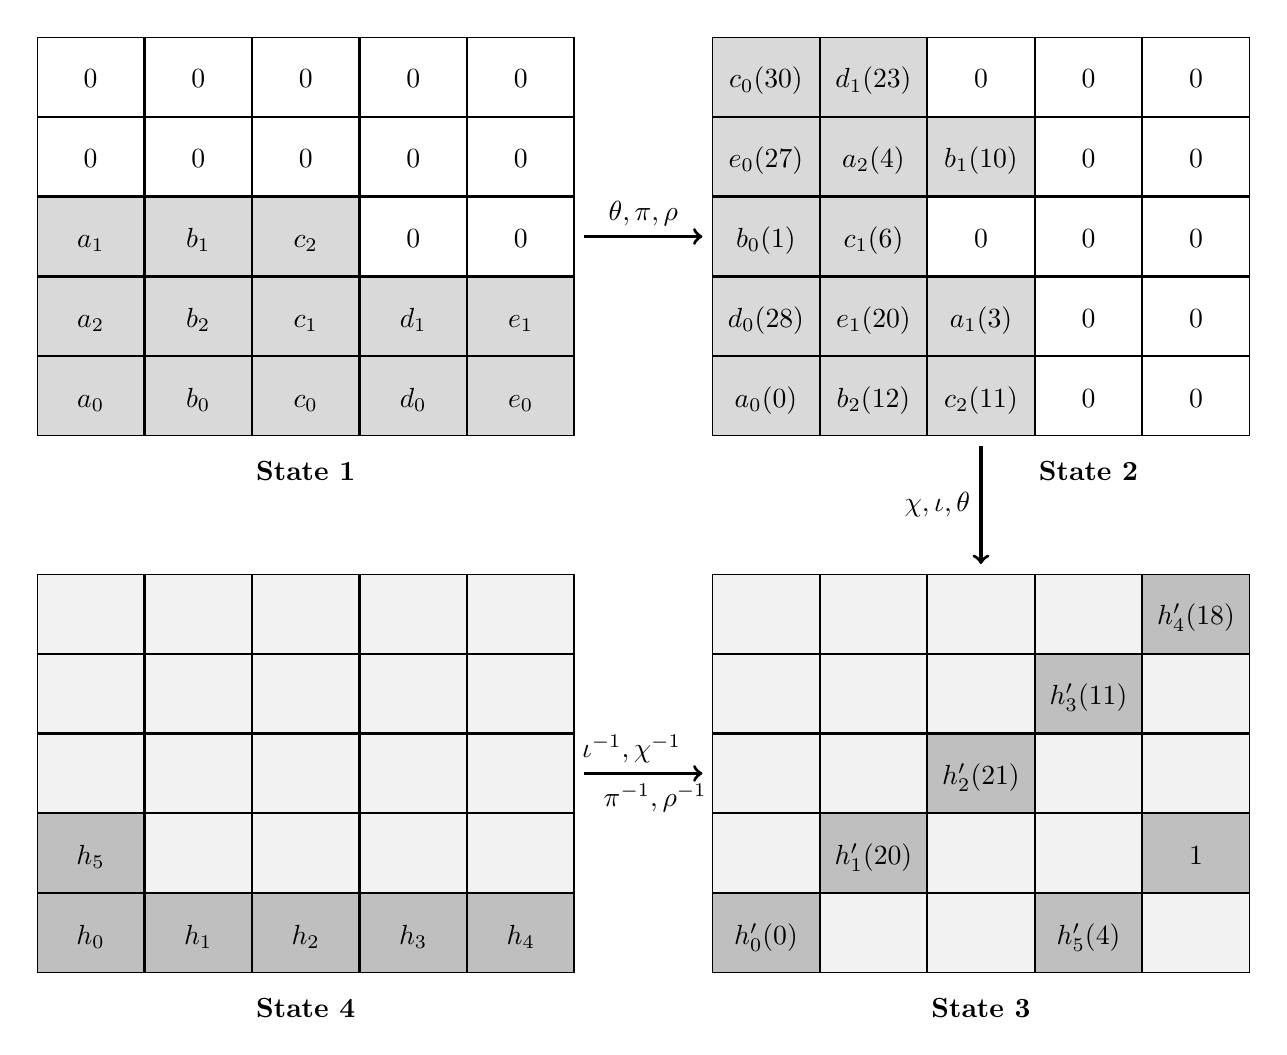
\begin{tikzpicture}[ampersand replacement=\&, scale=0.5]
			\matrix (am1) [matrix of nodes,nodes in empty cells,
			nodes={inner sep=5pt,text width=1.0cm,align=center,minimum height=1.0cm, draw,text height=1em,text depth=.2em},
			myrow/.list={(1,white),(2,white),(4,gray!30),(5,gray!30)},
			mycell/.list={(3,1,gray!30),(3,2,gray!30),(3,3,gray!30),(3,4,white),(3,5,white)}]    
			{
				$0$ \& $0$\& $0$ \& $0$ \& $0$\\
				$0$ \& $0$\& $0$ \& $0$ \& $0$\\
				$a_1$ \& $b_1$\& $c_2$ \& $0$ \& $0$\\
				$a_2$ \& $b_2$\& $c_1$ \& $d_1$ \& $e_1$\\
				$a_0$ \& $b_0$\& $c_0$ \& $d_0$ \& $e_0$\\
			};
			\matrix (am2) [right=1.5 cm of am1,matrix of nodes,nodes in empty cells,
			nodes={inner sep=5pt,text width=1.0cm,align=center,minimum height=1.0cm, draw,text height=1em,text depth=.2em},
			mycolumn/.list={(1,gray!30),(2,gray!30),(4,white),(5,white)},
			mycell/.list={(1,3,white),(3,3,white),(2,3,gray!30),(4,3,gray!30),(5,3,gray!30)}
			]    
			{
				$c_0(30)$ \& $d_1(23)$ \& $0$         \& $0$ \& $0$\\
				$e_0(27)$ \& $a_2(4)$ \& $b_1(10)$ \& $0$ \& $0$\\
				$b_0(1)$  \& $c_1(6)$  \& $0$         \& $0$ \& $0$\\
				$d_0(28)$ \& $e_1(20)$ \& $a_1(3)$  \& $0$ \& $0$\\
				$a_0(0)$  \& $b_2(12)$ \& $c_2(11)$ \& $0$ \& $0$\\
			};
			
			\matrix (am3) [below=1.5 cm of am2,matrix of nodes,nodes in empty cells,
			nodes={inner sep=5pt,text width=1.0cm,align=center,minimum height=1.0cm, draw,text height=1em,text depth=.2em, fill=gray!10},
			mycell/.list={(5,1,gray!50),(4,2,gray!50),(3,3,gray!50),(2,4,gray!50),(1,5,gray!50),(5,4,gray!50),(4,5,gray!50)}
			]    
			{
				\&      \&       \&      \& $h_4^\prime(18)$\\
				\&      \&       \&$h_3^\prime(11)$ \&         \\
				\&      \& $h_2^\prime(21)$\&      \&         \\
				\&$h_1^\prime(20)$ \&       \&      \& $1$        \\
				$h_0^\prime(0)$ \&         \&      \& $h_5^\prime(4)$     \&         \\
			};
			\matrix (am4) [left=1.50 cm of am3,matrix of nodes,nodes in empty cells,
			nodes={inner sep=5pt,text width=1.0cm,align=center,minimum height=1.0cm, draw,text height=1em,text depth=.2em, fill=gray!10},
			mycell/.list={(5,1,gray!50),(5,2,gray!50),(5,3,gray!50),(5,4,gray!50),(5,5,gray!50),(4,1,gray!50)}
			]    
			{
				\&  \&   \&  \& \\
				\&  \&   \&  \& \\
				\&  \&   \&  \& \\
				$h_5$ \&  \&   \&  \& \\
				$h_0$ \& $h_1$\& $h_2$ \& $h_3$ \& $h_4$\\
			};
			
			\node[ below=0.2cm of am1-5-3]{\bf State~1};
			\node[ below=0.2cm of am2-5-4]{\bf State~2};
			\node[ below=0.2cm of am3-5-3]{\bf State~3};
			\node[ below=0.2cm of am4-5-3]{\bf State~4};
			\draw[->, very thick] (am1)-- node[above]{$\theta, \pi,\rho$} (am2);
			\draw[->, very thick] (am2)-- node[left]{$\chi, \iota,\theta$} (am3);
			\draw[->, very thick] (am4)-- node[above, pos=0.4]{$\iota^{-1},\chi^{-1}$} node[below, pos=0.6]{$ \pi^{-1},\rho^{-1}$} (am3);
			\end{tikzpicture}
		}
		\caption{Preimage attack on $2$-round \KECCAK{}$[r:=800-384,\; c:=384]$ \label{atk}}
	\end{center}
\end{figure}

\end{frame}



%---------------------------------------------------------------
\begin{frame}{State 2 to State 3}
\begin{figure}
\begin{center}
	\resizebox{\textwidth}{!}{%
		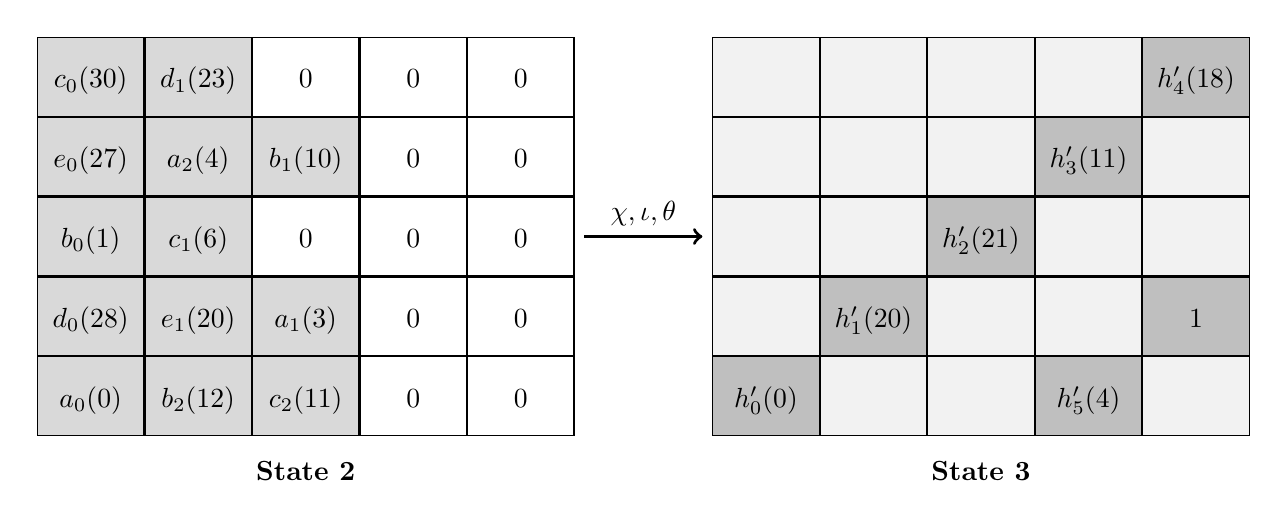
\begin{tikzpicture}[ampersand replacement=\&, scale=0.5]
		
		\matrix (am2) [matrix of nodes,nodes in empty cells,
		nodes={inner sep=5pt,text width=1.0cm,align=center,minimum height=1.0cm, draw,text height=1em,text depth=.2em},
		mycolumn/.list={(1,gray!30),(2,gray!30),(4,white),(5,white)},
		mycell/.list={(1,3,white),(3,3,white),(2,3,gray!30),(4,3,gray!30),(5,3,gray!30)}
		]	
		{
			$c_0(30)$ \& $d_1(23)$ \& $0$ 		\& $0$ \& $0$\\
			$e_0(27)$ \& $a_2(4)$ \& $b_1(10)$ \& $0$ \& $0$\\
			$b_0(1)$  \& $c_1(6)$  \& $0$ 		\& $0$ \& $0$\\
			$d_0(28)$\& $e_1(20)$ \& $a_1(3)$  \& $0$ \& $0$\\
			$a_0(0)$  \& $b_2(12)$ \& $c_2(11)$ \& $0$ \& $0$\\
		};
		
		\matrix (am3) [right=1.5 cm of am2,matrix of nodes,nodes in empty cells,
		nodes={inner sep=5pt,text width=1.0cm,align=center,minimum height=1.0cm, draw,text height=1em,text depth=.2em, fill=gray!10},
		mycell/.list={(5,1,gray!50),(4,2,gray!50),(3,3,gray!50),(2,4,gray!50),(1,5,gray!50),(5,4,gray!50),(4,5,gray!50)}
		]	
		{
			\&  	\&   	\&  \& $h_4^\prime(18)$ \\
			\&  	\&   	\&$h_3^\prime(11)$ \& 	\\
			\&  	\& $h_2^\prime(21)$\&  	\& 		\\
			\&$h_1^\prime(20)$ \&   \&  \& $1$		\\
			$h_0^\prime(0)$ \& \& \& $h_5^\prime(4)$ \& 	\\
		};
		
		\node[ below=0.2cm of am2-5-3]{\bf State~2};
		\node[ below=0.2cm of am3-5-3]{\bf State~3};
		
		\draw[->, very thick] (am2)-- node[above]{$\chi, \iota,\theta$} (am3);
		\end{tikzpicture}
	}
	\caption{Intermediate States in $2$-round preimage attack on \KECCAK{}$[r:=800-384,\; c:=384]$ \label{atk_partial}}
\end{center}
\end{figure}
\end{frame}


%----------------------------------------------------------------

\begin{frame}{Description of Attack}
\begin{itemize}

\item In state $1$, we initially have $13\cdot 32$ variables.
\pause
\medskip
\item In the state $3$, there are $7$ lanes whose values are fixed, this will impose a total of $7\cdot 32$ conditions.
\medskip
\item We also set $6$ conditions on the initial state (Equation~\ref{cond_state1}). This will further add $6 \cdot 32$ conditions.
\pause
\medskip
\item The number of variables and the number of conditions are equal. 
\pause
\medskip
\item So, we expect a solution.
\end{itemize}

\end{frame}

%-----------------------------------------------------------
\begin{frame}{Description of Attack}
\begin{itemize}
\item In state $3$, the values of $i^{\rm\;th}$-slice depend on the $(i-1)^{\rm th}$ and $i^{\rm\;th}$-slice of state $2$.
\medskip
\pause
\item First, we find the set of input message bits which satisfy the small collection of consecutive slices of state $3$.
\medskip
\pause
\item Then, we merge the solutions to find message bits which satisfy large collection of consecutive slices.

\end{itemize}
\end{frame}

\begin{frame}
	\frametitle{Attack Layout}
	\begin{itemize}
		\item We need to find values of variables in initial state for all the $32$ slices.
		\medskip
		\pause
		\item We solve for first $24$ slices and then solve for the remaining $8$ slices.
		\medskip
		\pause
		\item Solving for first $24$ slices:
		\medskip
			\begin{itemize}
				\item Find solutions for $8$ groups of $3$ slices.
				\medskip
				\pause
				\item Merge consecutive $3$ slices to get solutions for $6$ slices i.e. $4$ groups of $6$ slices.
				\medskip
				\pause
				\item Merge consecutive $6$ slices to get solutions for $12$ slices i.e. $2$ groups of $12$ slices.
				\medskip
				\pause
				\item Merge the two groups of $12$ slices to get solutions for $24$ slices.
			\end{itemize}
	\end{itemize}
\end{frame}

\begin{frame}
	\frametitle{Attack Layout}
	\begin{itemize}
		\item Solving for remaining $8$ slices:
		\medskip
		\pause
		\begin{itemize}
			\item Find solutions for the first $6$ slices.
			\medskip
			\pause
			\item Find solutions for the remaining $2$ slices.
			\medskip
			\pause
			\item Merge the above two groups to obtain solutions for the $8$ slices.			
			\medskip
			\pause
		\end{itemize}
		\item The last step of the attack is to merge solutions of the $24$ slices and $8$ slices.
		\medskip
		\pause
		\item Finally, we obtain a solution for all the $32$ slices.
	\end{itemize}
\end{frame}

%---------------------------------------------------------------
\begin{frame}{Possible solutions for groups of $3$ slices}
\begin{itemize}

\item Consider a group of $3$ slices (for example take the first $3$ slices).
\medskip
\pause
\item It contains the following message bits:
\medskip
\begin{itemize}
\item $a_0[0,1,2],\;\;a_1[3,4,5],\;\;a_2[4,5,6]$
\item $b_0[1,2,3],\;\; b_1[10,11,12],\;\;b_2[12,13,14]$
\item $c_0[30,31,0],\;\;c_1[6,7,8],\;\;c_2[11,12,13]$
\item $e_0[27,28,29],\;\; e_1[20,21,22]$
\end{itemize}
\medskip
\pause
\item Once we fix these message bits in the state~$2$, the slice~$1$ and slice~$2$ of state~$3$ get fixed.
\medskip
\pause
\item Furthermore, there is no dependency between these message bits.
\medskip
\pause
\item Thus, the total number of possible solutions for this $3$-slice are $2^{33-2\cdot 7}=2^{19}$.
\end{itemize}
\end{frame}


%------------------------------------------------------------------
\begin{frame}{Possible solutions for groups of 6 slices }
\begin{itemize}
\item This is obtained by merging two groups of $3$ slices.
\pause
\item Consider, for example, the first two $3$-slices (first $6$ slices).
\item  It contains the following message bits:
\begin{itemize}
\item $a_0[0-5],\;\;a_1[3-8],\;\;a_2[4-9]$
\item $b_0[1-6],\;\; b_1[10-15],\;\;b_2[12-17]$
\item $c_0[30-3],\;\;c_1[6-11],\;\;c_2[11-16]$
\item $e_0[27-0],\;\; e_1[20-25]$
\end{itemize}
\pause
\item During merging, we get to compute the bit values of slice~$3$ of the state~$3$ as well.
\pause
\item We already have the correct bit values of slice~$3$ of the state~$3$, and there is dependency between the above message bit variables.
\pause
\item The total number of possible solutions are $2^{2 \cdot 19 - 2 - 7}=2^{29}$.
\item There is dependency between bits $a_0[4,5], a_1[4,5]$ and $a_2[4,5]$.
\end{itemize}
\end{frame}

%-----------------------------------------------------------------
\begin{frame}{Possible solutions for groups of 12 slices}
\begin{itemize}
\item Similar to the case of $6$-slice, the solution for a $12$-slice is obtained by merging two $6$-slices.
\pause
\item Consider, for example, the first $12$ slices. It contains the following message bits:
\begin{itemize}
\item $a_0[0-11],\;\;a_1[3-14],\;\;a_2[4-15]$
\item $b_0[1-12],\;\; b_1[10-21],\;\;b_2[12-23]$
\item $c_0[30-9],\;\;c_1[6-17],\;\;c_2[11-22]$
\item $e_0[27-6],\;\; e_1[20-31]$
\end{itemize}
\pause
\item As before, here we again get the values of slice~$6$ of state~$3$. 
\pause
\item Similar to $6$-slice, the bit variables are dependent.

\item The bit variables $a_0,a_1,a_2[6-9], b_0,b_1,b_2[12]$, and $e_0,e_1[27-31]$ are dependent.
\pause
\item Hence, the total number of possible solutions are $2^{2 \cdot 29-10-7}=2^{41}$.
\end{itemize}
\end{frame}
%-----------------------------------------------------------------
\begin{frame}{Possible solutions for groups of $24$ slices}
\begin{itemize}
\item This is obtained by merging two groups of $12$ slices.
\medskip
\pause
\item For example, consider the first $24$ slices i.e., 
\medskip
\begin{itemize}
\item $a_0[0-23],\;\;a_1[3-26],\;\;a_2[4-27]$
\item $b_0[1-24],\;\; b_1[10-1],\;\;b_2[12-3]$
\item $c_0[30-21],\;\;c_1[6-29],\;\;c_2[11-2]$
\item $e_0[27-18],\;\; e_1[20-11]$
\end{itemize}
\medskip
\pause
\item This is very much similar to the $12$~slice solution.
\medskip
\item In this case, we get $34$ dependencies.
\medskip
\item The total number of possible solutions are $2^{2 \cdot 41-34-7}=2^{41}$.
\end{itemize}
\end{frame}


%-----------------------------------------------------------------

%--------------------------------------------------------------------
\begin{frame}{Final solutions}
\begin{itemize}
\item Using the same method, we find the possible solutions for the remaining $6$ slices and $2$ slices.
\medskip
\pause
\item For finding the solution for the last consecutive $8$ slices, we merge possible solution of its constituent $6$-slice and $2$-slice.
\medskip
\pause
\item Final solution space is obtained by merging the solution space of first $24$ slices and the last $8$ slices.
\medskip
\pause
\item In merging, we can compute the $\theta$ mapping of
the remaining two slices, in turn, we get the additional restriction of $2\cdot 7$ bits.
\medskip
\pause
\item In this case, we get $61$ dependencies.
\medskip
\item Total number of solutions are $2^{41 + 34 - 61 - 2\cdot 7} = 2^0 = 1$.
\end{itemize}

\end{frame}

\begin{frame}
	\frametitle{Attack Complexity}
	\begin{itemize}
		\item Space complexity of the attack = $2^{42}$
		\bigskip
		\item Time complexity of the attack = $2^{44}$
		\bigskip
		\item Also, we can find second preimages by setting $d_0$, $d_1$ to a constant such that it satisfies $d_0\left[i\right]=d_1\left[i\right]$ and then repeating the attack for this setting.
	\end{itemize}
\end{frame}

\section{Conclusion}

\begin{frame}{Conclusion}
\begin{itemize}
\item We have presented a preimage attack on the 2 rounds of round reduced \KECCAK$[r:=800-384, c:=384]$.
\medskip
\pause
\item This is a practical attack with attack complexity of $2^{44}$.
\medskip
\pause
\item Future work: Variant(s) of this attack for more rounds of \KECCAK.
\end{itemize}

\end{frame}

\begin{frame}{Questions?}
\centering{\huge{Thank You} 
}
\end{frame}

\end{document}
